\documentclass[11pt,a4paper]{report}
\usepackage[textwidth=37em,vmargin=30mm]{geometry}
\usepackage{calc,xunicode,amsmath,amssymb,paralist,enumitem,tabu,booktabs,datetime2,xeCJK,xeCJKfntef,listings}
\usepackage{tocloft,fancyhdr,tcolorbox,xcolor,graphicx,eso-pic,xltxtra,xelatexemoji}

\newcommand{\envyear}[0]{2025}
\newcommand{\envdatestr}[0]{2025-03-20}
\newcommand{\envfinaldir}[0]{webdb/2025/20250320/final}

\usepackage[hidelinks]{hyperref}
\hypersetup{
    colorlinks=false,
    pdfpagemode=FullScreen,
    pdftitle={Web Digest - \envdatestr}
}

\setlength{\cftbeforechapskip}{10pt}
\renewcommand{\cftchapfont}{\rmfamily\bfseries\large\raggedright}
\setlength{\cftbeforesecskip}{2pt}
\renewcommand{\cftsecfont}{\sffamily\small\raggedright}

\setdefaultleftmargin{2em}{2em}{1em}{1em}{1em}{1em}

\usepackage{xeCJK,xeCJKfntef}
\xeCJKsetup{PunctStyle=plain,RubberPunctSkip=false,CJKglue=\strut\hskip 0pt plus 0.1em minus 0.05em,CJKecglue=\strut\hskip 0.22em plus 0.2em}
\XeTeXlinebreaklocale "zh"
\XeTeXlinebreakskip = 0pt


\setmainfont{Brygada 1918}
\setromanfont{Brygada 1918}
\setsansfont{IBM Plex Sans}
\setmonofont{JetBrains Mono NL}
\setCJKmainfont{Noto Serif CJK SC}
\setCJKromanfont{Noto Serif CJK SC}
\setCJKsansfont{Noto Sans CJK SC}
\setCJKmonofont{Noto Sans CJK SC}

\setlength{\parindent}{0pt}
\setlength{\parskip}{8pt}
\linespread{1.15}

\lstset{
	basicstyle=\ttfamily\footnotesize,
	numbersep=5pt,
	backgroundcolor=\color{black!5},
	showspaces=false,
	showstringspaces=false,
	showtabs=false,
	tabsize=2,
	captionpos=b,
	breaklines=true,
	breakatwhitespace=true,
	breakautoindent=true,
	linewidth=\textwidth
}






\newcommand{\coverpic}[2]{
    % argv: itemurl, authorname
    Cover photo by #2~~(\href{#1}{#1})
}
\newcommand{\makeheader}[0]{
    \begin{titlepage}
        % \newgeometry{hmargin=15mm,tmargin=21mm,bmargin=12mm}
        \begin{center}
            
            \rmfamily\scshape
            \fontspec{BaskervilleF}
            \fontspec{Old Standard}
            \fontsize{59pt}{70pt}\selectfont
            WEB\hfill DIGEST
            
            \vfill
            % \vskip 30pt
            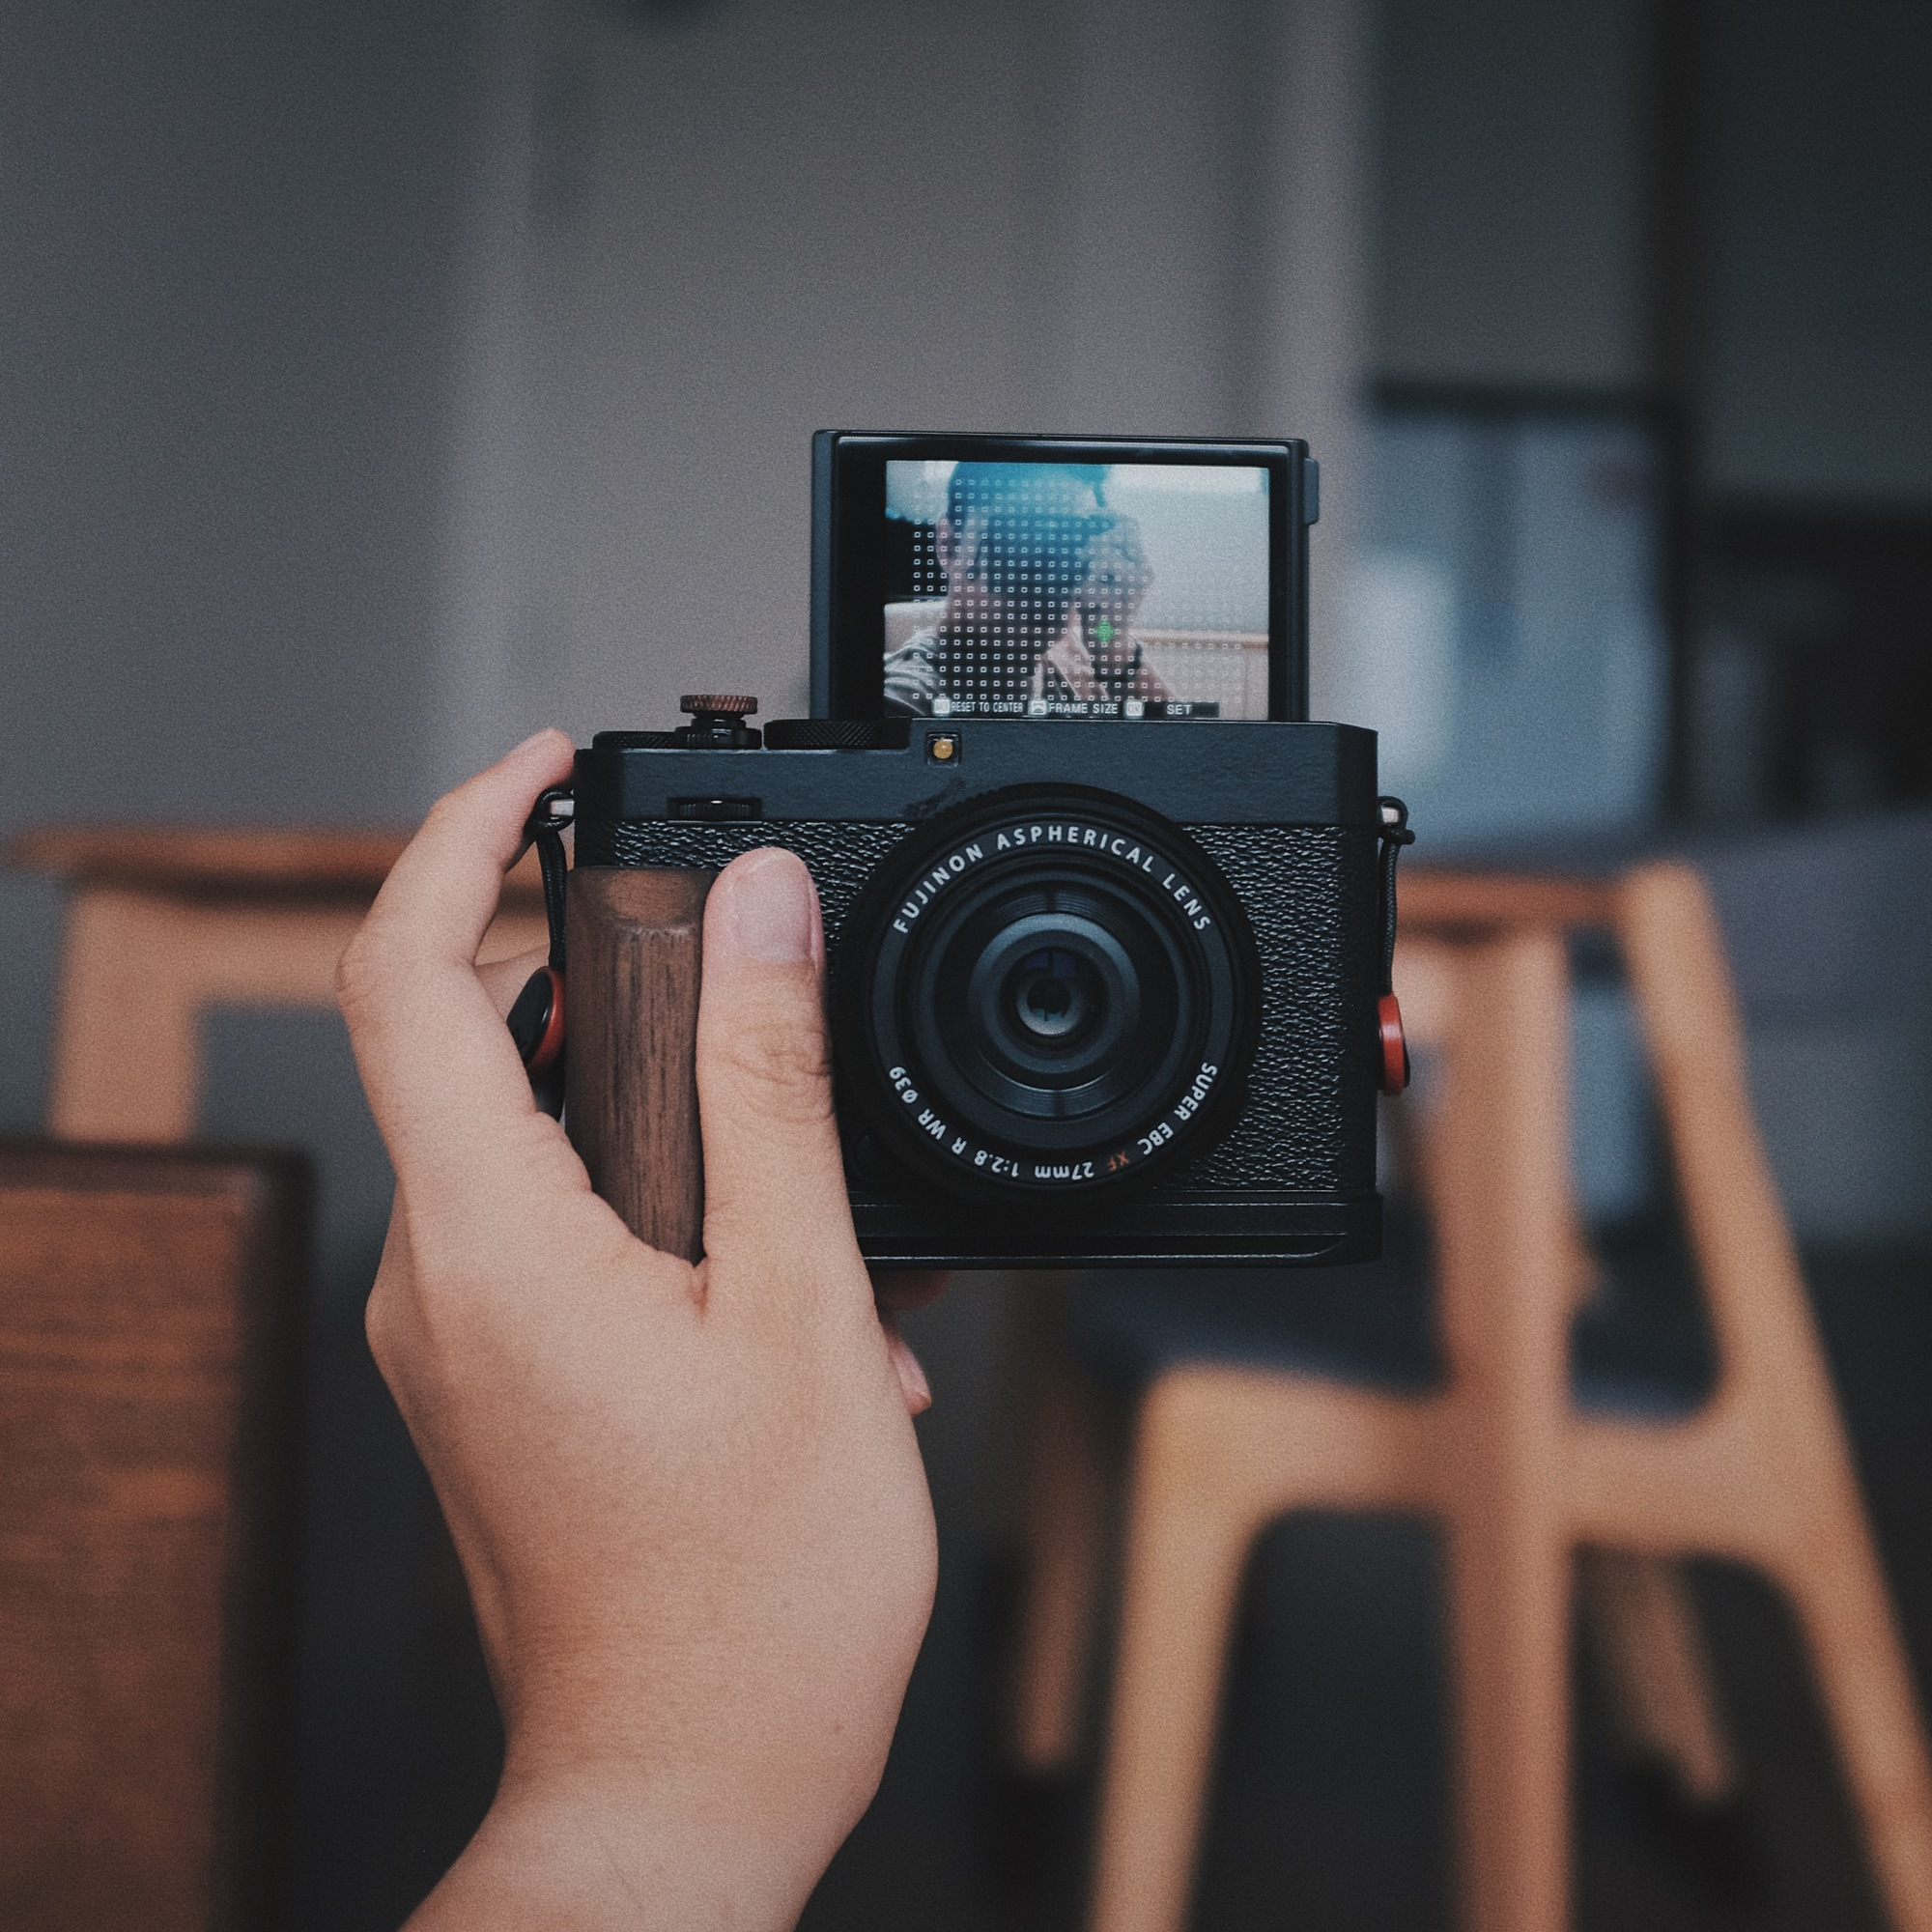
\includegraphics[width=\linewidth]{\envfinaldir/coverpic-prod.jpg}\par
            % \vskip 30pt
            \vfill

            \normalsize\rmfamily\scshape
            \copyright{} The Web Digest Project \hfill\large \envdatestr
        \end{center}
    \end{titlepage}
    % \restoregeometry
}
\newcommand{\simplehref}[1]{%
    \textcolor{blue!80!green}{\href{#1}{#1}}%
}
\renewcommand{\contentsname}{\center\Huge\sffamily\bfseries Contents\par\vskip 20pt}
\newcounter{ipartcounter}
\setcounter{ipartcounter}{0}
\newcommand{\ipart}[1]{
    % \vskip 20pt
    \clearpage
    \stepcounter{ipartcounter}
    \phantomsection
    \addcontentsline{toc}{chapter}{#1}
    % \begin{center}
    %     \Huge
    %     \sffamily\bfseries
    %     #1
    % \end{center}
    % \vskip 20pt plus 7pt
}
\newcounter{ichaptercounter}
\setcounter{ichaptercounter}{0}
\newcommand{\ichapter}[1]{
    % \vskip 20pt
    \clearpage
    \stepcounter{ichaptercounter}
    \phantomsection
    \addcontentsline{toc}{section}{\numberline{\arabic{ichaptercounter}}#1}
    \begin{center}
        \Huge
        \sffamily\bfseries
        #1
    \end{center}
    \vskip 20pt plus 7pt
}
\newcommand{\entrytitlefont}[1]{\subsection*{\raggedright\Large\sffamily\bfseries#1}}
\newcommand{\entryitemGeneric}[2]{
    % argv: title, url
    \parbox{\linewidth}{
        \entrytitlefont{#1}\par\vskip 5pt
        \footnotesize\ttfamily\mdseries
        \simplehref{#2}
    }\vskip 11pt plus 11pt minus 1pt
}
\newcommand{\entryitemGithub}[3]{
    % argv: title, url, desc
    \parbox{\linewidth}{
        \entrytitlefont{#1}\par\vskip 5pt
        \footnotesize\ttfamily\mdseries
        \simplehref{#2}\par\vskip 5pt
        \small\rmfamily\mdseries#3
    }\vskip 11pt plus 11pt minus 1pt
}
\newcommand{\entryitemAp}[3]{
    % argv: title, url, desc
    \parbox{\linewidth}{
        \entrytitlefont{#1}\par\vskip 5pt
        \footnotesize\ttfamily\mdseries
        \simplehref{#2}\par\vskip 5pt
        \small\rmfamily\mdseries#3
    }\vskip 11pt plus 11pt minus 1pt
}
\newcommand{\entryitemHackernews}[3]{
    % argv: title, hnurl, rawurl
    % \parbox{\linewidth}{
    %     \entrytitlefont{#1}\par\vskip 5pt
    %     \footnotesize\ttfamily\mdseries
    %     \simplehref{#3}\par
    %     \textcolor{black!50}{\href{#2}{#2}}
    % }\vskip 11pt plus 11pt minus 1pt
    \begin{minipage}{\linewidth}
            \entrytitlefont{#1}\par\vskip 5pt
            \footnotesize\ttfamily\mdseries
            \simplehref{#3}\par
            \textcolor{black!50}{\href{#2}{#2}}
    \end{minipage}\par\vskip 11pt plus 11pt minus 1pt
}







\begin{document}

\makeheader

\tableofcontents\clearpage




\ipart{Developers}
\ichapter{Hacker News}
\entryitemTwoLinks{Pierogi in Space}{https://news.ycombinator.com/item?id=43416302}{https://www.esa.int/Science\_Exploration/Human\_and\_Robotic\_Exploration/Pierogi\_in\_space}

\entryitemTwoLinks{Fauna Service Winding Down}{https://news.ycombinator.com/item?id=43414742}{https://fauna.com/blog/the-future-of-fauna}

\entryitemTwoLinks{AI Blindspots – Blindspots in LLMs I've noticed while AI coding}{https://news.ycombinator.com/item?id=43414393}{https://ezyang.github.io/ai-blindspots/}

\entryitemTwoLinks{Fine-tune Google's Gemma 3}{https://news.ycombinator.com/item?id=43414235}{https://unsloth.ai/blog/gemma3}

\entryitemTwoLinks{How fast the days are getting longer}{https://news.ycombinator.com/item?id=43413935}{https://joe-antognini.github.io/astronomy/daylight}

\entryitemTwoLinks{Memory safety for web fonts}{https://news.ycombinator.com/item?id=43413125}{https://developer.chrome.com/blog/memory-safety-fonts}

\entryitemTwoLinks{Video game workers in North America now have an industry-wide union}{https://news.ycombinator.com/item?id=43411934}{https://www.engadget.com/big-tech/video-game-workers-in-north-america-now-have-an-industry-wide-union-130024730.html}

\entryitemTwoLinks{Supply constraints do not explain house price, quantity growth across US cities}{https://news.ycombinator.com/item?id=43411258}{https://www.nber.org/papers/w33576}

\entryitemTwoLinks{Konva.js - Declarative 2D Canvas for React, Vue, and Svelte}{https://news.ycombinator.com/item?id=43410988}{https://konvajs.org/}

\entryitemTwoLinks{The Origin of the Pork Taboo}{https://news.ycombinator.com/item?id=43410885}{https://archaeology.org/issues/march-april-2025/letters-from/on-the-origin-of-the-pork-taboo/}

\entryitemTwoLinks{fd: A simple, fast and user-friendly alternative to 'find'}{https://news.ycombinator.com/item?id=43410692}{https://github.com/sharkdp/fd}

\entryitemTwoLinks{Tesla loses ground as Chinese EVs dominate global markets}{https://news.ycombinator.com/item?id=43410579}{https://restofworld.org/2025/tesla-loses-ground-chinese-ev-dominate-global-markets/}

\entryitemTwoLinks{I'm the Canadian who was detained by ICE for two weeks}{https://news.ycombinator.com/item?id=43410548}{https://www.theguardian.com/us-news/2025/mar/19/canadian-detained-us-immigration-jasmine-mooney}

\entryitemTwoLinks{Apple Loses Top Court Fight Over German Antitrust Crackdown}{https://news.ycombinator.com/item?id=43410247}{https://www.bloomberg.com/news/articles/2025-03-18/apple-loses-top-court-fight-against-german-antitrust-crackdown}

\entryitemTwoLinks{The Lost Art of Research as Leisure}{https://news.ycombinator.com/item?id=43410061}{https://kasurian.com/p/research-as-leisure}

\entryitemTwoLinks{The Internet Slum: is abandoning the Internet the next big thing? (2004)}{https://news.ycombinator.com/item?id=43409028}{https://www.fourmilab.ch/documents/netslum/}

\entryitemTwoLinks{CVE-2024-9956 – PassKey Account Takeover in All Mobile Browsers}{https://news.ycombinator.com/item?id=43408674}{https://mastersplinter.work/research/passkey/}

\entryitemTwoLinks{Crew-9 Returns to Earth}{https://news.ycombinator.com/item?id=43408540}{https://www.spacex.com/launches/mission/?missionId=crew-9-return}

\entryitemTwoLinks{Make Ubuntu packages 90\% faster by rebuilding them}{https://news.ycombinator.com/item?id=43406710}{https://gist.github.com/jwbee/7e8b27e298de8bbbf8abfa4c232db097}

\entryitemTwoLinks{Nvidia Dynamo: A Datacenter Scale Distributed Inference Serving Framework}{https://news.ycombinator.com/item?id=43404858}{https://github.com/ai-dynamo/dynamo}\ichapter{Phoronix}
\entryitemGeneric{\hskip 0pt{}SoftBank Acquiring ARM Server CPU Vendor Ampere Computing}{https://www.phoronix.com/news/SoftBank-Acquiring-Ampere}

\entryitemGeneric{\hskip 0pt{}Fedora 43 Hopes To Set An Expectation That Package Builds Are Reproducible}{https://www.phoronix.com/news/Fedora-43-Expect-Reproducible}

\entryitemGeneric{\hskip 0pt{}GNOME 48 Released With New Default Font, HDR Support, New Audio Player \& More}{https://www.phoronix.com/news/GNOME-48-Released}

\entryitemGeneric{\hskip 0pt{}Another Round Of Rust Compiler Improvements Merged For GCC 15.1}{https://www.phoronix.com/news/More-Rust-Merged-GCC-15.1}

\entryitemGeneric{\hskip 0pt{}Intel Wrapping Up Family 18 / Family 19 CPU Model Preparations Ahead Of Linux 6.15}{https://www.phoronix.com/news/Intel-FMV-Finishing-Linux-6.15}

\entryitemGeneric{\hskip 0pt{}Beyond The ROCm Software, AMD Has Been Making Great Strides In Documentation \& Robust Containers}{https://www.phoronix.com/review/amd-rocm-docs-containers-2025}

\entryitemGeneric{\hskip 0pt{}Intel AVX10 Drops Optional 512-bit: No AVX10 256-bit Only E-Cores In The Future}{https://www.phoronix.com/news/Intel-AVX10-Drops-256-Bit}

\entryitemGeneric{\hskip 0pt{}Linux 6.15 To Support The Airoha NPU - A RISC-V Network Processor Unit}{https://www.phoronix.com/news/Linux-6.15-Airoha-NPU}

\entryitemGeneric{\hskip 0pt{}DRM Sync Object Optimizations Show Minor Benefit On The Steam Deck}{https://www.phoronix.com/news/DRM-Sync-Obj-Optimizations-Deck}\ichapter{Dribbble}
\entryitemGeneric{\hskip 0pt{}Puzzle Fintech UI/UX design, User Interface experience}{https://dribbble.com/shots/25652036-Puzzle-Fintech-UI-UX-design-User-Interface-experience}

\entryitemGeneric{\hskip 0pt{}Novascan}{https://dribbble.com/shots/25790443-Novascan}

\entryitemGeneric{\hskip 0pt{}Crypto Bridge}{https://dribbble.com/shots/25783744-Crypto-Bridge}

\entryitemGeneric{\hskip 0pt{}Eclipse - Logo Design}{https://dribbble.com/shots/25784396-Eclipse-Logo-Design}

\entryitemGeneric{\hskip 0pt{}Cargo Shipment App UI}{https://dribbble.com/shots/25784159-Cargo-Shipment-App-UI}

\entryitemGeneric{\hskip 0pt{}Burn Bright, Take Flight}{https://dribbble.com/shots/25778930-Burn-Bright-Take-Flight}

\entryitemGeneric{\hskip 0pt{}Rose Logo Design [for sale]}{https://dribbble.com/shots/25775027-Rose-Logo-Design-for-sale}

\entryitemGeneric{\hskip 0pt{}Mammut Logo Redesign Concept}{https://dribbble.com/shots/25776663-Mammut-Logo-Redesign-Concept}

\entryitemGeneric{\hskip 0pt{}Cimet Logo Grid}{https://dribbble.com/shots/25710567-Cimet-Logo-Grid}

\entryitemGeneric{\hskip 0pt{}Glide wallet}{https://dribbble.com/shots/25768771-Glide-wallet}

\entryitemGeneric{\hskip 0pt{}Bento grid \& dashboard for revops startup}{https://dribbble.com/shots/25765472-Bento-grid-dashboard-for-revops-startup}

\entryitemGeneric{\hskip 0pt{}DL}{https://dribbble.com/shots/25775198-DL}

\entryitemGeneric{\hskip 0pt{}bigbeardamian: Badge Design}{https://dribbble.com/shots/25737398-bigbeardamian-Badge-Design}

\entryitemGeneric{\hskip 0pt{}Abstract S Logo Design // For Sale}{https://dribbble.com/shots/25764643-Abstract-S-Logo-Design-For-Sale}

\entryitemGeneric{\hskip 0pt{}Protec Recovery Logo Design}{https://dribbble.com/shots/25764203-Protec-Recovery-Logo-Design}

\entryitemGeneric{\hskip 0pt{}Spin}{https://dribbble.com/shots/25765149-Spin}

\entryitemGeneric{\hskip 0pt{}Fintech icons pack part 3 for download}{https://dribbble.com/shots/25728645-Fintech-icons-pack-part-3-for-download}

\entryitemGeneric{\hskip 0pt{}Capobara}{https://dribbble.com/shots/25764582-Capobara}

\entryitemGeneric{\hskip 0pt{}Triceratops}{https://dribbble.com/shots/25761010-Triceratops}

\entryitemGeneric{\hskip 0pt{}Tab Bar Animation}{https://dribbble.com/shots/25760227-Tab-Bar-Animation}

\entryitemGeneric{\hskip 0pt{}Chief Logo Design Process}{https://dribbble.com/shots/25759736-Chief-Logo-Design-Process}

\entryitemGeneric{\hskip 0pt{}World Clock App Design}{https://dribbble.com/shots/25760174-World-Clock-App-Design}

\entryitemGeneric{\hskip 0pt{}Flare - Logo Design 2}{https://dribbble.com/shots/25760645-Flare-Logo-Design-2}

\entryitemGeneric{\hskip 0pt{}Columbus Lions®}{https://dribbble.com/shots/25761563-Columbus-Lions}


\ipart{Developers~~~~(zh-Hans)}
\ichapter{Solidot}
\entryitemGeneric{\hskip 0pt{}Gemini 2.0 Flash 让任何人都能 PS}{https://www.solidot.org/story?sid=80830}

\entryitemGeneric{\hskip 0pt{}PC 玩家 92\% 的时间是在老游戏上}{https://www.solidot.org/story?sid=80829}

\entryitemGeneric{\hskip 0pt{}人类语言至少在 13.5 万年就存在}{https://www.solidot.org/story?sid=80828}

\entryitemGeneric{\hskip 0pt{}西班牙政治家对女性诉求的回应少于男性}{https://www.solidot.org/story?sid=80827}

\entryitemGeneric{\hskip 0pt{}SystemRescue 12.00 释出}{https://www.solidot.org/story?sid=80826}

\entryitemGeneric{\hskip 0pt{}Google 以 320 亿美元收购安全公司 Wiz}{https://www.solidot.org/story?sid=80825}

\entryitemGeneric{\hskip 0pt{}Eric Migicovsky 宣布推出两款运行 PebbleOS 的智能手表产品}{https://www.solidot.org/story?sid=80824}

\entryitemGeneric{\hskip 0pt{}密码复用攻击泛滥成灾}{https://www.solidot.org/story?sid=80823}

\entryitemGeneric{\hskip 0pt{}波音 Starliner 宇航员返回地面}{https://www.solidot.org/story?sid=80822}

\entryitemGeneric{\hskip 0pt{}欧洲科技公司呼吁欧盟推动购买欧洲科技产品}{https://www.solidot.org/story?sid=80821}

\entryitemGeneric{\hskip 0pt{}人类的脑力已经越过峰值?}{https://www.solidot.org/story?sid=80820}

\entryitemGeneric{\hskip 0pt{}周五是否应该成为新的周六?}{https://www.solidot.org/story?sid=80819}

\entryitemGeneric{\hskip 0pt{}哈佛对年收入 20 万美元以内家庭免除学费}{https://www.solidot.org/story?sid=80818}

\entryitemGeneric{\hskip 0pt{}百度副总裁的未成年女儿被指参与开盒}{https://www.solidot.org/story?sid=80817}

\entryitemGeneric{\hskip 0pt{}Google 在 AI 训练数据集的版权问题上与 OpenAI 意见一致}{https://www.solidot.org/story?sid=80816}

\entryitemGeneric{\hskip 0pt{}特斯拉二手车价格下跌}{https://www.solidot.org/story?sid=80815}

\entryitemGeneric{\hskip 0pt{}华为计划在 Windows 授权过期后转向 Linux}{https://www.solidot.org/story?sid=80814}

\entryitemGeneric{\hskip 0pt{}网信办等发布《人工智能生成合成内容标识办法》}{https://www.solidot.org/story?sid=80813}

\entryitemGeneric{\hskip 0pt{}GIMP 3.0 释出}{https://www.solidot.org/story?sid=80812}

\entryitemGeneric{\hskip 0pt{}Gemini 将在今年晚些时候取代 Google Assistant}{https://www.solidot.org/story?sid=80811}\ichapter{V2EX}
\entryitemGeneric{\hskip 0pt{}[职场话题] 有大龄 phper 吗?杭州,能一起做项目的小伙伴。}{https://www.v2ex.com/t/1119753}

\entryitemGeneric{\hskip 0pt{}[程序员] 多久掌握一个语言 or 框架是正常的}{https://www.v2ex.com/t/1119752}

\entryitemGeneric{\hskip 0pt{}[程序员] 豆瓣网页版小宇宙}{https://www.v2ex.com/t/1119751}

\entryitemGeneric{\hskip 0pt{}[问与答] 今年找工作好难,失业的你,每天都在干嘛呢?}{https://www.v2ex.com/t/1119750}

\entryitemGeneric{\hskip 0pt{}[问与答] 感觉自己的心态更适合做研究,请问有类似的朋友吗?}{https://www.v2ex.com/t/1119749}

\entryitemGeneric{\hskip 0pt{}[分享创造] 做了个「暴躁东北老妹儿」AI 塔罗师!免费!准!狠!}{https://www.v2ex.com/t/1119748}

\entryitemGeneric{\hskip 0pt{}[问与答] 如何把 google 搜索结果页面变成双列?}{https://www.v2ex.com/t/1119747}

\entryitemGeneric{\hskip 0pt{}[分享创造] 我做了一个在线尺子测量的工具站,做着玩,纯公益无广告}{https://www.v2ex.com/t/1119746}

\entryitemGeneric{\hskip 0pt{}[Local LLM] 一块 4090,怎么来评估部署大模型后(假设为 DeepSeek-R1-Distill-Qwen-7B)的并发数?、、}{https://www.v2ex.com/t/1119745}

\entryitemGeneric{\hskip 0pt{}[Apple] 关于 iOS/iPadOS 上 YouTube APP 检测网速很慢的问题}{https://www.v2ex.com/t/1119744}

\entryitemGeneric{\hskip 0pt{}[职场话题] 应届生简历工作年限该怎么填?}{https://www.v2ex.com/t/1119743}

\entryitemGeneric{\hskip 0pt{}[Apple] mac studio 那个配置最具性价比?}{https://www.v2ex.com/t/1119742}

\entryitemGeneric{\hskip 0pt{}[程序员] 相亲经历:跨行业相处的思考}{https://www.v2ex.com/t/1119741}

\entryitemGeneric{\hskip 0pt{}[Google] [长期] GoogleVoice 靓号+1 拖 2-3-4 永久号(无需保号)}{https://www.v2ex.com/t/1119740}

\entryitemGeneric{\hskip 0pt{}[分享发现] 我做了一个 avif 转 png 的小工具: https://aviftopng.top}{https://www.v2ex.com/t/1119739}

\entryitemGeneric{\hskip 0pt{}[酷工作] [北京]外企招聘前端/后端/PM/UI}{https://www.v2ex.com/t/1119738}

\entryitemGeneric{\hskip 0pt{}[问与答] 因公司内网限制,只能使用 openrouter 访问国外主流闭源大模型,该如何充值}{https://www.v2ex.com/t/1119737}

\entryitemGeneric{\hskip 0pt{}[分享发现] 两台笔记本的生产力最大化}{https://www.v2ex.com/t/1119736}

\entryitemGeneric{\hskip 0pt{}[问与答] 如何优雅地吃汉堡🍔}{https://www.v2ex.com/t/1119735}

\entryitemGeneric{\hskip 0pt{}[问与答] 有道 dict.youdao.com/dictvoice?audio=xxx 文字朗读接口部分失效}{https://www.v2ex.com/t/1119732}

\entryitemGeneric{\hskip 0pt{}[分享创造] 免费小插件: 方便下载小红书无水印视频(rednoteapp.co)}{https://www.v2ex.com/t/1119731}

\entryitemGeneric{\hskip 0pt{}[推广] [长期] GoogleVoice 靓号+1 拖 2-3-4 永久号(无需保号)}{https://www.v2ex.com/t/1119729}

\entryitemGeneric{\hskip 0pt{}[问与答] 求助靠谱渠道从境内需要往俄罗斯银行 Sber 银行转账几万卢布}{https://www.v2ex.com/t/1119727}

\entryitemGeneric{\hskip 0pt{}[程序员] 看 windsurf 最新版本更新了 tab 能力,和 cursor 对比如何呢?}{https://www.v2ex.com/t/1119726}

\entryitemGeneric{\hskip 0pt{}[硬件] 求推荐个电源, NAS 用。}{https://www.v2ex.com/t/1119725}

\entryitemGeneric{\hskip 0pt{}[问与答] Mac mini M4 激活}{https://www.v2ex.com/t/1119724}

\entryitemGeneric{\hskip 0pt{}[Windows] 请教个问题, windows 明明我没开什么程序,为什么内存占用这么高}{https://www.v2ex.com/t/1119723}

\entryitemGeneric{\hskip 0pt{}[macOS] macbook 如何设置通过 自定义触控板手势(如四指轻点)来触发网页刷新操作(类似按 Command+R 刷新页面)}{https://www.v2ex.com/t/1119722}

\entryitemGeneric{\hskip 0pt{}[OpenAI] 本地部署 qwq 32b 回答很笨是什么原因}{https://www.v2ex.com/t/1119721}

\entryitemGeneric{\hskip 0pt{}[分享发现] realVNC viewer 导致的按键问题}{https://www.v2ex.com/t/1119719}

\entryitemGeneric{\hskip 0pt{}[职场话题] v 友们我现在怎么办}{https://www.v2ex.com/t/1119717}

\entryitemGeneric{\hskip 0pt{}[Notion] Notion 如何下载 APK}{https://www.v2ex.com/t/1119716}

\entryitemGeneric{\hskip 0pt{}[JavaScript] 如何在移动端 h5 页面实现<Select/>搜索下拉选择框!}{https://www.v2ex.com/t/1119715}

\entryitemGeneric{\hskip 0pt{}[远程工作] AI Agent 全栈开发工程师|海外电商 AI+SaaS 招长期远程兼职}{https://www.v2ex.com/t/1119714}

\entryitemGeneric{\hskip 0pt{}[全球工单系统] 有没有在蓝厂工作的研发 你们的手表太拉了}{https://www.v2ex.com/t/1119713}

\entryitemGeneric{\hskip 0pt{}[全球工单系统] 最近抖音的推荐算法出问题了?}{https://www.v2ex.com/t/1119712}

\entryitemGeneric{\hskip 0pt{}[问与答] [讨论] 想知道在这种情况下,各位 v 友觉得公道不}{https://www.v2ex.com/t/1119711}

\entryitemGeneric{\hskip 0pt{}[微信] 微信小程序上 提示用户前往淘宝或拼多多 违规吗?}{https://www.v2ex.com/t/1119709}

\entryitemGeneric{\hskip 0pt{}[职场话题] 兄弟们 offer 选择,求指点,}{https://www.v2ex.com/t/1119707}

\entryitemGeneric{\hskip 0pt{}[分享创造] 有用过 soul 里的连睡或者呼吸麦的吗}{https://www.v2ex.com/t/1119705}

\entryitemGeneric{\hskip 0pt{}[V2EX] v2ex 能否考虑增加``引用回复''的功能?}{https://www.v2ex.com/t/1119702}

\entryitemGeneric{\hskip 0pt{}[杭州] 有杭州的 v 友吗?天际线真的关了?}{https://www.v2ex.com/t/1119701}

\entryitemGeneric{\hskip 0pt{}[Apple] 大家在购买 Apple 产品的时候,哪些产品加购了 Applecare+啊?}{https://www.v2ex.com/t/1119700}

\entryitemGeneric{\hskip 0pt{}[游戏] 如何玩《开罗》系列游戏最舒服}{https://www.v2ex.com/t/1119697}

\entryitemGeneric{\hskip 0pt{}[程序员] OpenAI Agents SDK 与 Claude MCP 谁能笑到最后}{https://www.v2ex.com/t/1119696}

\entryitemGeneric{\hskip 0pt{}[Java] java8 的 springboot 漏洞那么多,留在 java8 不升级的话如何解决这些漏洞}{https://www.v2ex.com/t/1119695}

\entryitemGeneric{\hskip 0pt{}[中州韻] WSL Debian 2 安装 ibus-rime 总是没反应}{https://www.v2ex.com/t/1119693}

\entryitemGeneric{\hskip 0pt{}[职场话题] 非 CS 专业想当程序员,应该如何开始?}{https://www.v2ex.com/t/1119691}

\entryitemGeneric{\hskip 0pt{}[分享创造] 新闻联播 AI 解读}{https://www.v2ex.com/t/1119690}

\entryitemGeneric{\hskip 0pt{}[互联网] 求助: The connection for this site is not secure}{https://www.v2ex.com/t/1119688}


\ipart{Generic News}
\ichapter{AP News}
\entryitemWithDescription{\hskip 0pt{}Quirky livestream that lets viewers help fish is a hit with millions}{https://apnews.com/article/f09da0435a61e88a1d7b0372920bb7da}{}

\entryitemWithDescription{\hskip 0pt{}A former studio engineer is charged with stealing unreleased Eminem music and selling it online}{https://apnews.com/article/6b707ffbada116baf9c0042d12675244}{}

\entryitemWithDescription{\hskip 0pt{}Italian postal service sees surge in mail for Pope Francis, much sent from children}{https://apnews.com/article/5e9816ab53c4408aca7242312fed8734}{}

\entryitemWithDescription{\hskip 0pt{}Defense Department webpage on Jackie Robinson goes down, then returns amid DEI purge}{https://apnews.com/article/beed0c8883e7a31af0d9a71615cc643d}{}

\entryitemWithDescription{\hskip 0pt{}Burrow, Cousins and Goff will be featured on 2nd season of Netflix's `Quarterback' series}{https://apnews.com/article/87a3eec33c89a6ff1cee040562d1be6a}{}

\entryitemWithDescription{\hskip 0pt{}Ben \& Jerry's alleges parent company Unilever removed its CEO over social activism}{https://apnews.com/article/f0dfc60035b7a3e57e11421f5494c0c7}{}

\entryitemWithDescription{\hskip 0pt{}Mikey Madison, Jack Black and Jon Hamm will host spring `Saturday Night Live' episodes}{https://apnews.com/article/45c567f97f6e0eb6b777ce9d2678cc84}{}

\entryitemWithDescription{\hskip 0pt{}European Union lays out how Apple must open its tech up to competitors under bloc's digital rules}{https://apnews.com/article/8f1c2f1fda1d3ffeed50322df8093817}{}

\entryitemWithDescription{\hskip 0pt{}A 10-year-old boy in Tokyo ended up with Shohei Ohtani's first home run of the season}{https://apnews.com/article/31aac1f29c83bd130fe17f30babe125f}{}

\entryitemWithDescription{\hskip 0pt{}Mexico City bans violent bullfighting, sparking fury and celebration}{https://apnews.com/article/09707d6eddef807bc330fc286d7b1b15}{}

\entryitemWithDescription{\hskip 0pt{}The Doobie Brothers in 2025: A tour, a new album and a date with Songwriters Hall of Fame}{https://apnews.com/article/4f69e928422940f343da13ca374a0457}{}

\entryitemWithDescription{\hskip 0pt{}Blue Ghost lander captures stunning sunset shots on the moon before falling silent}{https://apnews.com/article/0bb0d0845dfe4b27a5affa52912fa8dc}{}

\entryitemWithDescription{\hskip 0pt{}Omaha Mavericks' trash (can) turns into treasure with program earning its first March Madness bid}{https://apnews.com/article/e885b944b7ede70326e0178f23eebcf5}{}






\clearpage
\leavevmode\vfill
\footnotesize

Copyright \copyright{} 2023-2025 Neruthes and other contributors.

This document is published with CC BY-NC-ND 4.0 license.

The entries listed in this newsletter may be copyrighted by their respective creators.

This newsletter is generated by the Web Digest project.

The newsletters are also delivered via Telegram channel \CJKunderline{\href{https://t.me/webdigestchannel}{https://t.me/webdigestchannel}}.\\
RSS feed is available at \CJKunderline{\href{https://webdigest.pages.dev/rss.xml}{https://webdigest.pages.dev/rss.xml}}.

This newsletter is available in PDF at
\CJKunderline{\href{https://webdigest.pages.dev/}{https://webdigest.pages.dev/}}.

The source code being used to generate this newsletter is available at\\
\CJKunderline{\href{https://github.com/neruthes/webdigest}{https://github.com/neruthes/webdigest}}.

This newsletter is also available in
\CJKunderline{\href{http://webdigest.pages.dev/readhtml/\envyear/WebDigest-20250320.html}{HTML}} and
\CJKunderline{\href{https://github.com/neruthes/webdigest/blob/master/markdown/\envyear/WebDigest-20250320.md}{Markdown}}.


\coverpic{https://unsplash.com/photos/an-aerial-view-of-a-beach-and-the-ocean-WlylrSgY3fo}{Daniel J. Schwarz}


\end{document}
